\section{Motivation}\label{sec:motivation}

It is well known that router administrator interfaces present an attack surface, allowing attackers to scan for vulnerabilities and reconfigure the router through malicious requests~\cite{niemietz2015owning,jeitner2022xdri}.
Unlike in a terrestrial setting, a satellite internet router is often part of a physical system including a motorized dish which can be affected.
However, these new routers are being implemented without the institutional memory of historic vulnerabilities and their mitigations, opening up new denial of service attacks through rotating the dish and overusing the motor.

We therefore assess the security of the Starlink user terminal, paying particular attention to the attack surface exposed by its web admin interface.
We explore both how requests are made to this interface and the effects of sending undocumented commands, through the use of a fuzzer capable of iterating through the unauthenticated command space.
Through this approach we find an exploit in the command decoding and execution logic which, when combined with commands affecting the state of the dish, result in denial of service persisting until the router is physically power-cycled.
This can be widely exploited due to poor security practices such as a lack of password authentication on the admin interface, or default passwords on the WiFi network itself.

This vulnerability was reported to Starlink, and a fix has been promptly deployed.

\begin{figure}
    \centering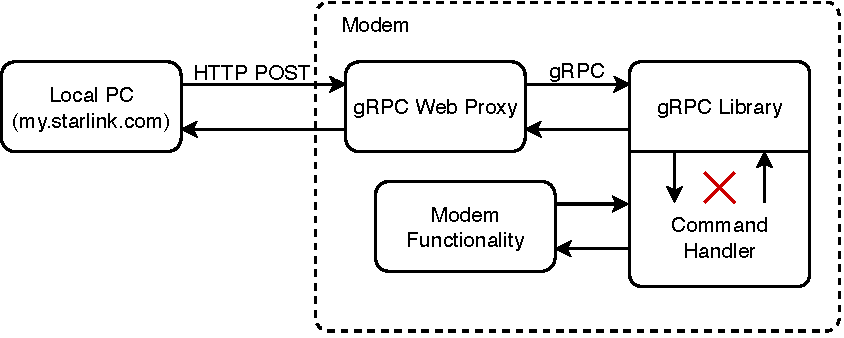
\includegraphics[width=\columnwidth]{img/modem.pdf}
    \caption{Overview of the Starlink modem functionality. gRPC calls are encapsulated within HTTP POST requests by the web interface, which are decoded and processed. Malformed gRPC requests cause the command handler to crash, resulting in the modem no longer being able to respond to commands.}
    \label{fig:modem}
    \vspace{-1em}
\end{figure}
